\chapter{Architectural Diagram}

We plan to utilize a basic client-server architecture to complete this project as shown in Figure~\ref{fig:arch}.

\begin{figure}[htb]
\centering
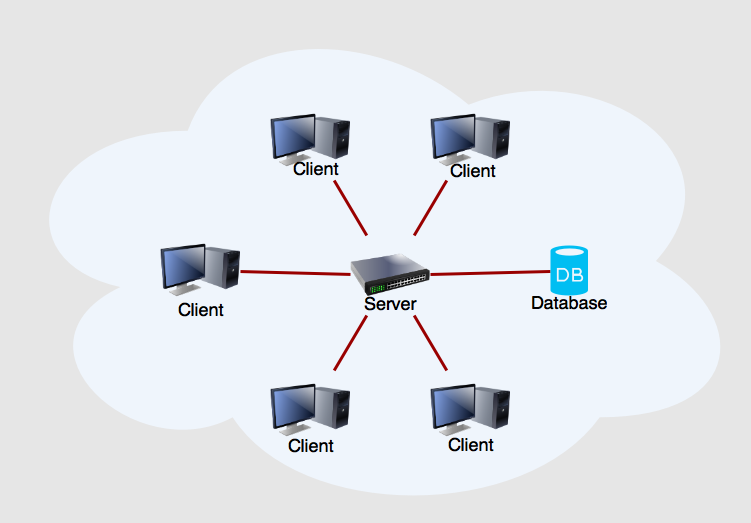
\includegraphics[width=\textwidth]{arch.png}
\caption{Client-Server Architecture}
\label{fig:arch}
\end{figure}

** FROM COEN 174 **
In our system, the users will include TAs, RAs, anyone in the approval process, and Scott Andrews. These users will be able to use an internet browser, acting as a client, in order to access our site. The server in our system will be hosted using Santa Clara University?s Engineering Design Center host. The server will be responsible for storing the form data for each student in the database and generating and sending the approval and rejection emails among those involved in the process. The database or datastore will be a file that the server will write to and read from in order to access data.